\section{Theorie}
\label{sec:Theorie}

Zwei über eine Kopplung verbundene Schwingsysteme werden gekoppelte Systeme genannt.
Wird eines der Systeme ausgelenkt, während das andere ruht, findet aufgrund der Kopplung ein Energieübertrag statt. Das ausgelenkte Systeme schwingt mit immer kleinerer Amplitude, bis es zum Stehen kommt, während 
das zunächst ruhende System mit immer größerer Amplitude schwingt. Dabei schwingt jedes System mit seiner Eigenfrequenz. Werden Energieverluste vernachlässigt, wiederholt sich dieser Vorgang immer wieder.

Im Folgenden werden zwei über einen Kopplungskondensator gekoppelte elekrische Schwingkreise betrachtet. Ein schematischer Aufbau des gekoppelten System ist in \autoref{fig:gekoppSchwingkreis} zu sehen.

\begin{figure}[H]
    \centering
    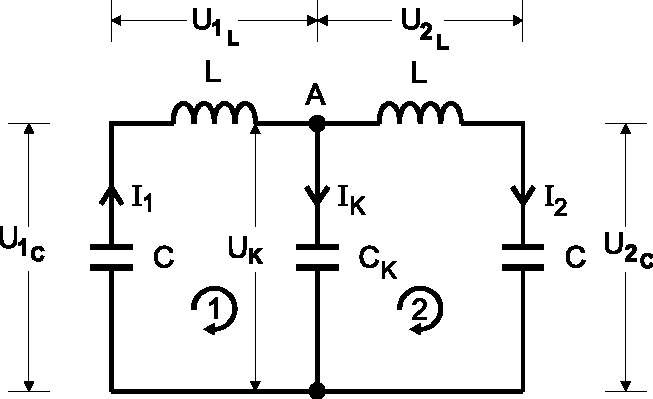
\includegraphics{SchwingkreisAbb.pdf}
    \caption{Schematische Darstellung eines gekoppelten Schwingkreises\cite{ap04}.}
    \label{fig:gekoppSchwingkreis}
\end{figure}

\newpage

\subsection{Schwingungsgleichungen gekoppelter Schwingkreise}

Mithilfe der Kirchhoffschen Knoten- und Maschenregel ergeben sich

\begin{align*}
    I_k &= I_1-I_2\, ,\\
    0   &= U_{1,C} + U_{1,L} + U_K\, , \\ 
    0   &= U_{2,C} + U_{2,L} + U_K\,.
\end{align*}

Mit 
\begin{equation*}
    U_C = \dfrac{1}{C} \int I \, \text{d}t
\end{equation*}
und
\begin{equation*}
    U_L = L \dot{I}
\end{equation*}
ergeben sich nach Differenzieren nach der Zeit
\begin{equation}
    L\ddot{I}_1 + \dfrac{1}{C}I_1 + \dfrac{1}{C_k}(I_1 - I_2) = 0
    \label{eq:DGL1}
\end{equation}
und
\begin{equation}
    L\ddot{I}_2 + \dfrac{1}{C}I_2 - \dfrac{1}{C_k}(I_1 - I_2) = 0\,.
    \label{eq:DGL2}
\end{equation}

Werden nun \eqref{eq:DGL1} und \eqref{eq:DGL2} voneinander addiert bzw. subtrahiert, entstehen zwei lineare Differentialgleichungen mit den Variablen $I_1+I_2$ bzw. $I_1-I_2$.
Es folgen
\begin{equation}
    L \,\diff{^2}{t^2}(I_1+I_2) + \dfrac{1}{C}(I_1 + I_2) = 0
    \label{eq:addDGL}
\end{equation}
und
\begin{equation}
    L \,\diff{^2}{t^2}(I_1 - I_2) + \left(\dfrac{1}{C} + \dfrac{2}{C_k} \right)(I_1 - I_2) = 0\,.
\end{equation}

\newpage

Als homogene Differentialgleichungen des harmonischen Oszillators sind die Lösungen gegeben durch

\begin{equation}
    (I_1+I_2)(t) = I_{0,+} \cos(ω_+t)
    \label{eq:gleiSchwi}
\end{equation}
mit 
\begin{align*}
    I_{0,+} &= I_{1,0}+I_{2,0}\, , \\
    ω_+     &=\dfrac{1}{\sqrt{LC}}
\end{align*}
sowie

\begin{equation*}
    (I_1-I_2)(t) = I_{0,-}\cos(ω_-t)
    \label{eq:gegSchwi}
\end{equation*}
mit 
\begin{align*}
    I_{0,-} &=I_{1,0} - I_{2,0}\, , \\
    ω_-     &= \dfrac{1}{\sqrt{L \left(\dfrac{1}{C}+\dfrac{2}{C_k}\right)^{-1}}}\,.
\end{align*} \\

Aus \eqref{eq:gleiSchwi} und \eqref{eq:gegSchwi} lassen sich nun Lösungen für $I_1(t)$ und $I_2(t)$ bestimmen, die sich zu
\begin{equation}
    I_1(t) = \dfrac{1}{2}(I_{0,+}\cos(ω_+ t) + I_{0,-}\cos(ω_- t))
\end{equation}
und
\begin{equation}
    I_2(t) = \dfrac{1}{2}(I_{0,+}\cos(ω_+ t) - I_{0,-}\cos(ω_- t))
\end{equation}
ergeben. \\

Ist nun $I_{1,0} = I_{2,0}$, ist auch $I_{0,-} = 0$, $I_1(t)$ und $I_2(t)$ schwingen zu jedem Zeitpunkt $t$ mit der Frequenz $ν_+ = \dfrac{1}{2πω_+}$ in Phase und es gilt
\begin{equation*}
     I_1(t) = I_2(t) = I_0 \cos(ω_+ t)\,.
\end{equation*}

Analog ergibt sich für eine gegenphasige Schwingung, also $I_{1,0} = -I_{2,0}$, $I_{0,+}=0$ und damit
\begin{equation*}
    I_1(t) = I_0 \cos(ω_- t) = -I_2(t)\,.
\end{equation*}
Dabei schwingt das System mit der erhöhten Frequenz $ν_- = \dfrac{1}{2πω_-}$. Die gleich- und gegenphasigen Schwingungen des gekoppelten Systems werden als Fundamentalschwingungen bezeichnet.

Es lässt sich ein weiterer Spezialfall beobachten. Wird eine der beiden Startamplituden, hier $I_{2,0}$, auf null gesetzt, während die andere verschieden von null ist, stellt sich eine gekoppelte Schwingung ein.
Die Stromverläufe ergeben sich dann zu
\begin{equation}
    I_1(t) = \dfrac{1}{2} I_{1,0}(\cos(ω_+ t) + \cos(ω_- t))
    \label{eq:gekoSchwi1}
\end{equation}
und
\begin{equation}
    I_2(t) = \dfrac{1}{2} I_{1,0}(\cos(ω_+ t) - \cos(ω_- t))\,.
    \label{eq:gekoSchwi2}
\end{equation}

Unter Anwendung von
\begin{equation*}
    \cos(a) + \cos(b) = 2 \cos(\dfrac{1}{2}(a+b)) \cos(\dfrac{1}{2}(a-b))
\end{equation*} 

\begin{equation*}
    \cos(a) - \cos(b) = 2 \sin(\dfrac{1}{2}(a+b)) \sin(\dfrac{1}{2}(a-b))
\end{equation*} 

lassen sich \eqref{eq:gekoSchwi1} und \eqref{eq:gekoSchwi2} zu
\begin{equation*}
    I_1(t) = I_{1,0}\cos(\dfrac{1}{2}(ω_+ + ω_-)t) \cos(\dfrac{1}{2}(ω_+ - ω_-)t) 
\end{equation*}
und
\begin{equation*}
    I_2(t) = I_{1,0}\sin(\dfrac{1}{2}(ω_+ + ω_-)t) \sin(\dfrac{1}{2}(ω_+ - ω_-)t)
\end{equation*}
vereinfachen. Wie zu erkennen ist, schwingt das System nun mit der Frequenz $ν_+ + ν_-$, die im Folgenden ungefähr mit der der Eigenfrequenz des einzelnen Schwingkreises übereinstimmen soll.
Dazu wird angenommen, dass $C_k >> C$ gilt und damit
\begin{align*}
    \dfrac{1}{2}(ω_+ + ω_- & \approx ω_+) \\
    ω_- - ω_+ & << ω_+
\end{align*}
Die Schwingungsamplitude oszilliert dabei mit der niedrigeren Frequenz $ν_- - ν_+$ zwischen $I_{1,0}$ und null. Dieser Prozess wird als Schwebung mit der Schwebungsfrequenz $ν_- - ν_+$ bezeichnet.
Eine schematische Darstellung einer solchen Schwebung ist in \autoref{fig:schwebung} zu betrachten.

\begin{figure}[H]
    \centering
    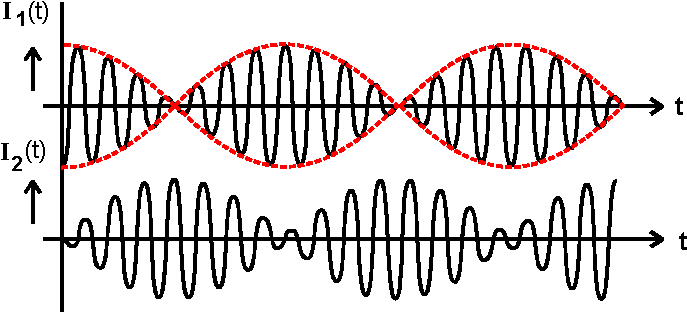
\includegraphics{SchwebungAbb.pdf}
    \caption{Stromverlauf in den Schwingkreisen bei einer Schwebung\cite{ap04}.}
    \label{fig:schwebung}
\end{figure}

\subsection{Frequenzabhängigkeit des Stromes eines gekoppelten Schwingkreises}

Wie in \autoref{fig:SinSchwingkreisAbb} dargestellt soll nun eine durch eine Sinusspannung erzwungende Schwingung des gekoppelten Schwingkreises betrachtet werden.
Die unvermeidbare Dämpfung, also alle potenziellen Energieverluste, werden durch ohmsche Widerstände in den beiden Hälften des Schwingkreises repräsentiert.

\begin{figure}
    \centering
    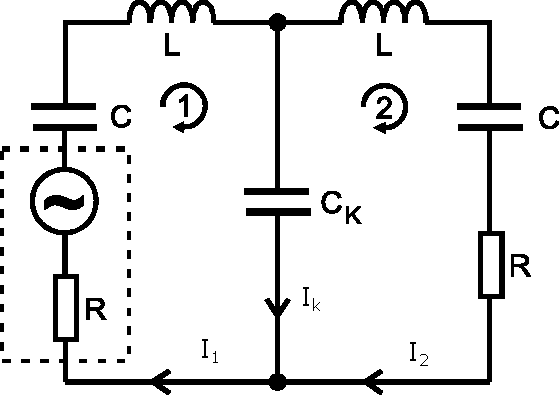
\includegraphics{SinSchwingkreisAbb.pdf}
    \caption{Gekoppelter Schwingkreis mit Verlustwiderständen $R$ und Sinusgenerator\cite{ap04}.}
    \label{fig:SinSchwingkreisAbb}
\end{figure}

Die Sinusspannung sei dabei gegeben durch
\begin{equation*}
    U = U_0 e^{iωt}\,.
\end{equation*}

Erneut lassen sich durch Anwendung der Kirchhoffschen Maschenregeln einige Beziehungen herleiten. So gelten

\begin{equation}
    (Z_C + Z_L + Z_R)I_1 - Z_{C_k}I_2 = U
\end{equation}
im ersten und
\begin{equation}
    (Z_C + Z_L + Z_R)I_2 -Z_{C_k}I_1 = 0
\end{equation}
im zweiten Schwingkreis mit 
\begin{align*}
    Z_C     &= -i\dfrac{1}{ωC}\,,   &  Z_L     &= iωL\,,  &   Z_R     &= R\,,   &    Z_{C_k} &= -i\dfrac{1}{ω C_k}\,.
\end{align*}

\newpage

Definiere
\begin{equation*}
    Z(ω) := ωL - \dfrac{1}{ω}\left(\dfrac{1}{C} + \dfrac{1}{C_k}\right)\,,
\end{equation*} dann lässt sich $I_2$, nach Trennung von Real- und Imaginärteil und Eliminierung von $I_1$, schreiben als

\begin{equation}
    I_2 = U \dfrac{-2 ω C_k R Z(ω) + i \left(-\dfrac{1}{ωC_k} + ω (C_k Z^2(ω) -  R^2 C_k) \right)}{4 ω^2 C^2_k R^2 Z^2(ω) + \left(\dfrac{1}{ω C_k} - ω (C_k Z^2(ω) +  R^2 C_k) \right)^2}\,
\end{equation} der Betrag ergibt sich dann zu

\begin{equation}
    |I_2| = |U| \dfrac{1}{\sqrt{4 ω^2 C^2_k R^2 Z^2(ω) + \left(\dfrac{1}{ω C_k} - ω (C_k Z^2(ω) +  R^2 C_k) \right)^2}} := |U||\mathcal{L}|
\end{equation} mit Leitwert $\mathcal{L}$.\\

Dieser Leitwert wird für die bereits berechneten Fundamentalfrequenzen des Systems extremal mit
\begin{align}
    |\mathcal{L}(ω_+)| = \dfrac{1}{R \sqrt{4+ \dfrac{R^2 C^2_k}{L C}}} \label{eq:Lomega+}\,, \\
    |\mathcal{L}(ω_-)| = \dfrac{1}{R \sqrt{4+ \dfrac{R^2 C^2_k}{L C} \left(1 + \dfrac{C}{C_k}\right)}} \label{eq:Lomega-}\,.
\end{align}

Dabei sind \eqref{eq:Lomega+} und \eqref{eq:Lomega-} klein gegen vier, sodass
\begin{equation*}
    |\mathcal{L}(ω_+)| \approx |\mathcal{L}(ω_-)| \approx \dfrac{2}{R} 
\end{equation*} als Näherung gilt.

Der Strom erreicht also bei beiden Fundamentalfrequenzen Maximalwerte, die näherungsweise gleich sind. Die beiden gekoppelten Schwingkreise lassen sich nun als ein einzelner Schwingkreis der Induktivität
\begin{equation*}
    L_{ges} = 2 L
\end{equation*} und der Kapazität 

\begin{equation*}
    C_{ges} = \dfrac{1}{\dfrac{1}{C} + \dfrac{1}{C}} = \dfrac{C}{2}
\end{equation*} betrachten, da die Frequenz $ν_+$ nicht von der Kopplungskapazität abhängt, also nahezu kein Strom durch die Kopplung fließen kann.
Dieser "doppelte" Schwingkreis besitzt nun die selbe Resonanzfrequenz wie die Einzelschwingkreise. 

% Therorie soweit fertig...